\documentclass{article}

% if you need to pass options to natbib, use, e.g.:
% \PassOptionsToPackage{numbers, compress}{natbib}
% before loading nips_2017
%
% to avoid loading the natbib package, add option nonatbib:
% \usepackage[nonatbib]{nips_2017}

\usepackage[final]{nips_2017}

% to compile a camera-ready version, add the [final] option, e.g.:
% \usepackage[final]{nips_2017}
\usepackage{enumerate}
\usepackage{ulem}
\usepackage[utf8]{inputenc} % allow utf-8 input
\usepackage[T1]{fontenc}    % use 8-bit T1 fonts
\usepackage{hyperref}       % hyperlinks
\usepackage{url}            % simple URL typesetting
\usepackage{booktabs}       % professional-quality tables
\usepackage{amsfonts}       % blackboard math symbols
\usepackage{nicefrac}       % compact symbols for 1/2, etc.
\usepackage{microtype}      % microtypography
\usepackage{cite}
\usepackage{amsmath}
\usepackage{graphicx} 
\usepackage{listings}
\usepackage{algorithm}  
\usepackage{algpseudocode}  
\usepackage{amsmath}  
\usepackage{xcolor}  	%高亮使用的颜色
\definecolor{commentcolor}{RGB}{85,139,78}
\definecolor{stringcolor}{RGB}{206,145,108}
\definecolor{keywordcolor}{RGB}{34,34,250}
\definecolor{backcolor}{RGB}{220,220,220}
\lstset{						%高亮代码设置
	language=python, 					%Python语法高亮
	linewidth=0.9\linewidth,      		%列表list宽度
	%basicstyle=\ttfamily,				%tt无法显示空格
	commentstyle=\color{commentcolor},	%注释颜色
	keywordstyle=\color{keywordcolor},	%关键词颜色
	stringstyle=\color{stringcolor},	%字符串颜色
	%showspaces=true,					%显示空格
	numbers=left,						%行数显示在左侧
	numberstyle=\tiny\emptyaccsupp,		%行数数字格式
	numbersep=5pt,						%数字间隔
	frame=single,						%加框
	framerule=0pt,						%不划线
	escapeinside=@@,					%逃逸标志
	emptylines=1,						%
	xleftmargin=3em,					%list左边距
	backgroundcolor=\color{backcolor},	%列表背景色
	tabsize=4,							%制表符长度为4个字符
	gobble=4							%忽略每行代码前4个字符
	}

\usepackage{accsupp}	
\newcommand{\emptyaccsupp}[1]{\BeginAccSupp{ActualText={}}#1\EndAccSupp{}}
\renewcommand{\algorithmicrequire}{\textbf{Input:}}  % Use Input in the format of Algorithm  
\renewcommand{\algorithmicensure}{\textbf{Output:}} % Use Output in the format of Algorithm  

\hypersetup{colorlinks,linkcolor={blue},citecolor={blue},urlcolor={blue}}  

\title{CS150 Database and Data Mining\\Course Project}

% The \author macro works with any number of authors. There are two
% commands used to separate the names and addresses of multiple
% authors: \And and \AND.
%
% Using \And between authors leaves it to LaTeX to determine where to
% break the lines. Using \AND forces a line break at that point. So,
% if LaTeX puts 3 of 4 authors names on the first line, and the last
% on the second line, try using \AND instead of \And before the third
% author name.

\author{
  Qiu Longtian\\
  ID: 2018533107\\
  \texttt{qiult@shanghaitech.edu.cn} \\
  %% examples of more authors
   \And
  Shi 	Qianjing\\
  ID: 2018533194\\
  \texttt{shiqj@shanghaitech.edu.cn}
  %% Coauthor \\
  %% Affiliation \\
  %% Address \\
  %% \texttt{email} \\
  %% \AND
  %% Coauthor \\
  %% Affiliation \\
  %% Address \\
  %% \texttt{email} \\
  %% \And
  %% Coauthor \\
  %% Affiliation \\
  %% Address \\
  %% \texttt{email} \\
  %% \And
  %% Coauthor \\
  %% Affiliation \\
  %% Address \\
  %% \texttt{email} \\
}

\begin{document}
% \nipsfinalcopy is no longer used

\maketitle


\section{Explore the dataset}
Before we train our model, we need to analyze the data.
In the original data set, the total 19 columns can be categorized into 2 types: categorical features, such as: Problem Hierarchy, Problem Name, etc, and numerical features, such as: Step End Time, Correct First Attempt and etc.And we will add new features by the original numerical features.
	\subsection{Data Structure:}
	For data separating, we found that Problem Hierarchy is a combination of Problem Unit and Problem Section. So it can be seperated to 2 parts. Therefore, there are 20 columns in all. And we have also found that the Opportunity is connected with $ \sim $$ \sim $ when it has more than one KC. We can separate them by $ \sim $$ \sim $.
	\subsection{Train Data:}
	The goal is to predict the answer of Correct First Attempt(CFA) for given data, so we just focus on the relation between CFA and other columns. For example, for CFA = 1, let's look at "Step Duration (sec)", which counts 181599. Mean is about 17.9 ,and std is about 35.2. 3rd quartile(Q3) is 17. So we may consider that if a student's Step Duration is larger than 53, his CFA is very likely be 0.

	\subsection{Test Data:}
	Since the training data is very comprehensive while some of them are useless in test data. In test data, only these columns have value, which are Row, Anon Student Id, Problem Hierarchy, Problem Name, Problem View, Step Name, Correct First Attempt, KC(Default), Opportunity(Default). 




\section{Data cleaning}
The first thing we do in data cleaning is to remove the meaningless columns and here is a list of columns which marks meaningless in this problem ["Row", "First Transaction Time", "Step Start Time", "Correct Transaction Time", "Step End Time", "Step Duration (sec)", "Error Step Duration (sec)", “Hints”]. These columns will not be used in following steps. For the rest of meaningful columns—— ["Anon Student Id", "Problem Hierarchy", "Problem Name", "Problem View", "Step Name", "Correct Step Duration (sec)", "Correct First Attempt", "Incorrects", “Corrects”, ”KC(Default)", “Opportunity(Default)”], we decide to pick out reasonable rows. \\
According to the “describe()” function in pandas library, we find there are two columns are meaningful but have outliers—["Correct Step Duration (sec)", “Incorrects”, “Corrects”]. The result of “describe()” function is shown in Figure1 and Figure2. 
\begin{figure}[h]
\begin{minipage}[t]{0.45\linewidth}
\centering
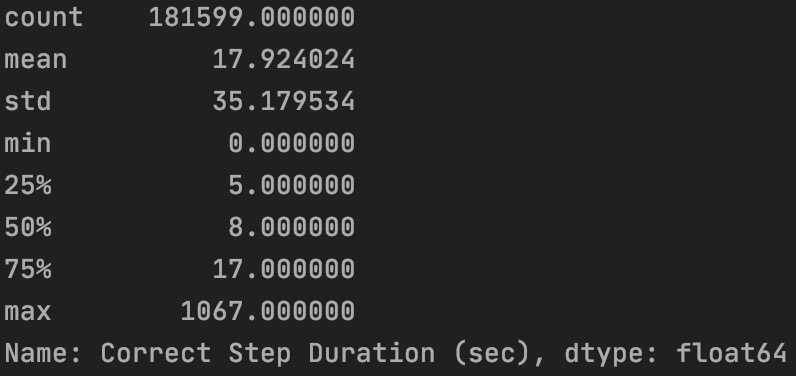
\includegraphics[width=5.5cm,height=3.5cm]{figure1.jpg}
\caption{Distribution of column CSD}
\end{minipage}
\begin{minipage}[t]{0.45\linewidth}        %图片占用一行宽度的45%
\hspace{2mm}
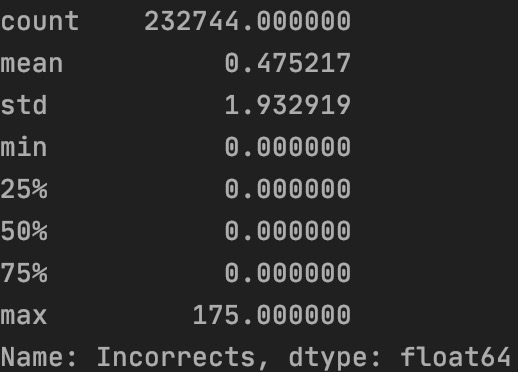
\includegraphics[width=5.5cm,height=3.5cm]{figure2.jpg}
\caption{Distribution of column Incorrects}
\end{minipage}
\end{figure}
So we decide to remove the outlier by the checking whether the delta of the value and it mean value is larger than 10 times its standard deviation. The formula is "if |value - mean of value| > standard deviation of value, then remove value". By this way, we removed about 800 rows in total.\\
Besides, we also check whether the data in a row is inconsistent. The rule for inconsistent is defined by observation. If the “Correct First Attempt” value of a row is 1, then the “Correct Step Duration (sec)” of the row is not a nan value. Any row violate the rule above will be marked as inconsistent and be removed. However, the result shows there is no inconsistent row in the training dataset.\\
Given the column “Problem Hierarchy” consist of two subpart—“Section” and “Unit”. We separate the column “Problem Hierarchy” into two columns—“Problem Section” and “Problem Unit”.\\
At last, after the training data is processed by our data cleaning, there are 11 columns remaining —['Anon Student Id', 'Problem Section’, ‘'Problem Unit’’, 'Problem Name', 'Problem View', 'Step Name', 'Correct Step Duration (sec)', 'Correct First Attempt', 'Incorrects', 'KC(Default)', 'Opportunity(Default)'].\\

\section{Feature engineering}
Feature engineering is the most important part in solving the problem. And we are trying to generate the most relevant features to the predicting column “Correct First Attempt” from the data in training data set.\\
Here we first deal with the categorial columns first. Nowadays there are several popular schema to encode categorial attributes, such as One-hot Encoding Scheme, Dummy Coding Scheme, Effect Coding Scheme, Bin-counting Scheme and Feature Hashing Scheme. Here we choose to try two of the schemas, which are One-hot Encoding Scheme and Feature Hashing Scheme. The implement of these two encode schema is done by the library in sklearn.feature\_extraction and sklearn.preprocessing. Then we explore the unique value of these categorial columns, the result is shown in Table 1.\\

\begin{table}[h]
\centering
\begin{tabular}{|c|c|c|c|c|}
\hline
Anon Student Id & Problem Section & Problem Unit & Problem Name & Step Name \\ \hline
174             & 138             & 32           & 1021         & 60624     \\ \hline
\end{tabular}
\caption{Unique number of categorial columns value}
\label{tab:my-table}
\end{table}

If we choose to do one hot encoding on all of the categorial columns, we will get 174*138*32*1021*60624 = 1.74e16 features, which is obviously too large to train, so we turn to “Feature Hashing Scheme” to get a fixed number of features. The actual number of feature generated by the hashing encoder is treated as an hyperparameter and will be decided later in ‘Hyperparameter selection and model performance’ section. After we generate features for categorial columns, we treat column “Problem View”directly as an feature since it’s value is related to the “Correct First Attempt”. Now we will process more complex columns—-“KC(Default)” and “Opportunity(Default)”. Since there may be more than one knowledge component and corresponding opportunity value in one row. First, we build up a table of difficulty of a knowledge component, the difficulty of a knowledge component is defined by $\frac{the\,number \,of \,rows\, where \,the \,knowledge \,component\, appear\, and \,the\, value\, of \,“Correct\, First \,Attempt\,” equals \,one}{ the\, number 
\,of \,rows\, where \,the\, knowledge\, component \,appear}$.\\
The result table is like a dictionary as shown in figure 3.

\begin{figure}[h]
\centering
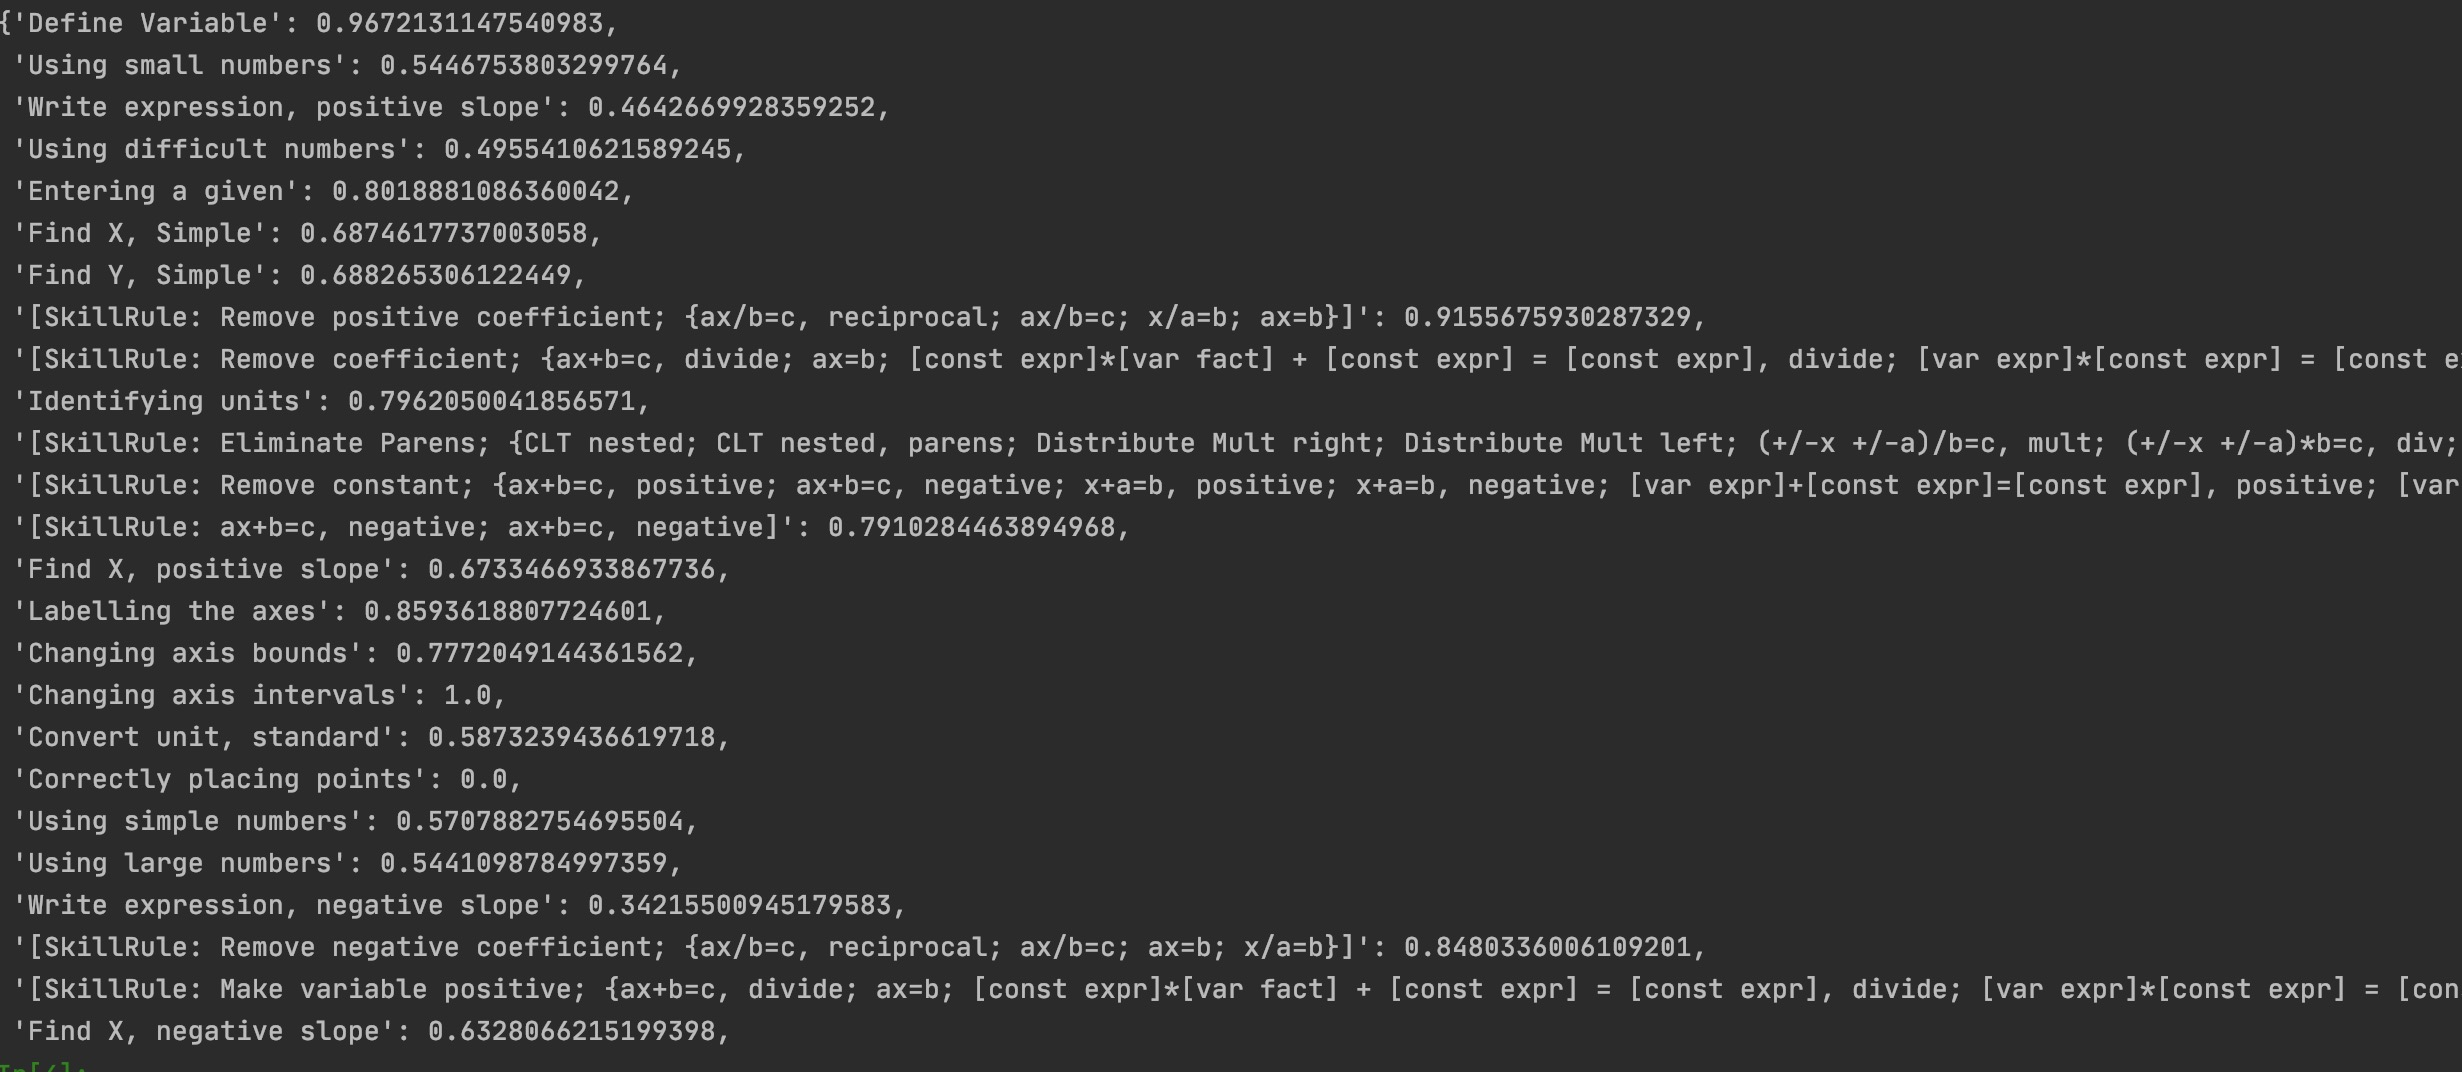
\includegraphics[width=12cm,height=5cm]{figure3.jpg}
\caption{Result table}
\end{figure}

Then we are able to generate a feature called knowledge difficulty based on our knowledge component difficulty table. To be more specific, the value of feature “knowledge difficulty” equals to the sum of knowledge components appear in the row divided by the number of knowledge component appear in the row. We also treat the number of knowledge component in a row as a feature either.\\
Opportunity is related to the knowledge component, so we generate a feature called opportunity value. Since there may be more than knowledge component and corresponding opportunity in one row, we defined opportunity value equals the sum of the difficulty of knowledge component times corresponding opportunity number, then divided the result by sum of opportunity numbers.$\frac{sum(KC\_i * OPPO\_i}{sum(OPPO\_i)}$, where KC\_i means ith knowledge component and OPPO\_i means ith opportunity number. If the knowledge component is not in the knowledge component difficulty table, we will assign the mean value of knowledge component difficulty table to it. Afterwards, we construct two table called person intelligent table and step difficulty table similar to knowledge difficulty table. The person intelligent table is designed to estimate how smart a participate is. The person intelligent table is defined by a function which takes mean values of one participate’s “"Correct Step Duration (sec)", "Correct First Attempt", “Incorrects" and “Corrects” and output a score.

\begin{figure}[h]
\centering
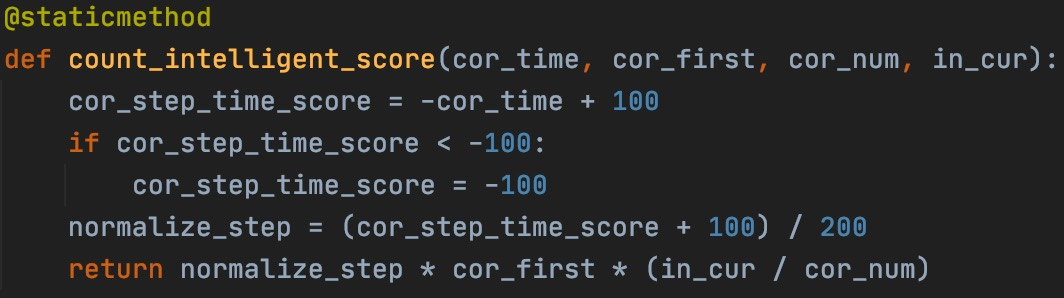
\includegraphics[width=12cm,height=5cm]{figure4.jpg}
\caption{Person intelligent table}
\end{figure}

With person intelligent table in figure 4, we generate the feature called person intelligent which is defined by the value of person intelligent table given an “Anon Student Id”. With respect to step difficulty table, it estimate the difficulty of a problem step which is defined by the number of rows one problem step appear and the value of “Correct First Attempt” equals 1 divided by the number of rows one problem step appear. Then we generate a feature called step difficulty based on the value of step difficulty table 
given a “Step Name”.\\
In conclusion, there are number of hash output * 5 + 5 features listed below.
	\begin{enumerate}[(1)]
	\item \textbf{Anon Student Id}
	\item \textbf{Problem Section}
	\item \textbf{Problem Unit}
	\item \textbf{Problem Name}
	\item \textbf{Step Name}
	\item \textbf{Knowledge Difficulty}
	\item \textbf{Person Intelligent}
	\item \textbf{Knowledge Component Number}
	\item \textbf{Step Difficulty}
	\item \textbf{Opportunity Value}
	\end{enumerate}

\section{Learning algorithm}

	\subsection{Learning Algorithm Methods and Description}
	After we have transformed some data into numerical data, we can start training and testing. After reading many papers, we have tried several methods for our prediction: AdaBoost classifie, GradientBoostingClassifier, BaggingClassifier, RandomForestClassifier, VotingClassifie, HistGradientBoostingRegressor, RandomForestRegressor, HistGradientBoostingRegressor, AdaBoostRegressor to know which one is better.

	\begin{enumerate}[(1)]
	\item AdaBoost classifier: An AdaBoost classifier is a meta-estimator that begins by fitting a classifier on the original dataset and then fits additional copies of the classifier on the same dataset but where the weights of incorrectly classified instances are adjusted such that subsequent classifiers focus more on difficult cases.
	
	\item GradientBoostingClassifier: GB builds an additive model in a forward stage-wise fashion; It allows for the optimization of arbitrary differentiable loss functions. 

	\item BaggingClassifier: A Bagging classifier is an ensemble meta-estimator that fits base classifiers each on random subsets of the original dataset and then aggregate their individual predictions (either by voting or by averaging) to form a final prediction. 

	\item RandomForestClassifier: A random forest is a meta estimator that fits a number of decision tree classifiers on various sub-samples of the dataset and uses averaging to improve the predictive accuracy and control over-fitting. 

	\item HistGradientBoostingRegressor: This estimator has native support for missing values (NaNs). During training, the tree grower learns at each split point whether samples with missing values should go to the left or right child, based on the potential gain. 

	\item RandomForestRegressor: A random forest is a meta estimator that fits a number of classifying decision trees on various sub-samples of the dataset and uses averaging to improve the predictive accuracy and control over-fitting. 

	\item HistGradientBoostingRegressor: This estimator is much faster than GradientBoostingRegressor for big datasets.

	\item AdaBoostRegressor: An AdaBoost regressor is a meta-estimator.

	\item RandomForestRegressor: A random forest is a meta estimator that fits a number of classifying decision trees on various sub-samples of the dataset and uses averaging to improve the predictive accuracy and control over-fitting.
	\end{enumerate}

	\subsection{Methods Result}
	And the RMSE result is shown in table 2.
	\begin{table}[h]
	\centering
	\begin{tabular}{|c|c|}
	\hline
	\textbf{Method}               & \textbf{RMSE} \\ \hline
	AdaBoost                      & 0.41222       \\ \hline
	GradientBoostingRegressor     & 0.41221       \\ \hline
	GradientBoosting              & 0.41404       \\ \hline
	Bagging                       & 0.44889       \\ \hline
	RandomForest                  & 0.42302       \\ \hline
	HistGradientBoostingRegressor & 0.39356       \\ \hline
	HistGradientBoosting          & 0.40856       \\ \hline
	AdaBoostRegressor             & 0.42480       \\ \hline
	RandomForestRegressor         & 0.44384       \\ \hline
	\end{tabular}
	\caption{The result of nine algorithms}
	\label{tab:my-table}
	\end{table}
	According to the performance of learning algorithm result , we decide to try combination of different algorithm. The implementation is realized by the function VotingRegressor(). The result is shown in table 3.
	\begin{table}[h]
	\centering
	\begin{tabular}{|c|c|}
	\hline
	GradientBoostingRegressor\&HistGradientBoostingRegressor & 0.40671 \\ \hline
	GradientBoostingRegressor\&RandomForestRegressor         & 0.41585 \\ \hline
	HistGradientBoostingRegressor\&RandomForestRegressor     & 0.39736 \\ \hline
	\end{tabular}
	\caption{The result of each combination}
	\label{tab:my-table}
	\end{table}


\section{Hyperparameter selection and model performance}	
The learning algorithm we choose is HistGradientBoostingRegressor which has the best performance among all the single or combination learning algorithm. And now we need to find the best hyperparameter for the HistGradientBoostingRegressor. The main parameters are loss function, learning rate, L2 regularization parameter, pseudo-random number generator to control the subsampling,  maximum number of iterations. The rest parameter will be remained as default value given by sklearn library. Since the inner relation between the parameters are unknown for us.  We adopt an random testing method. First we define the reasonable range for the hyperparameter. The range is shown in figure 5.

\begin{figure}[h]
\centering
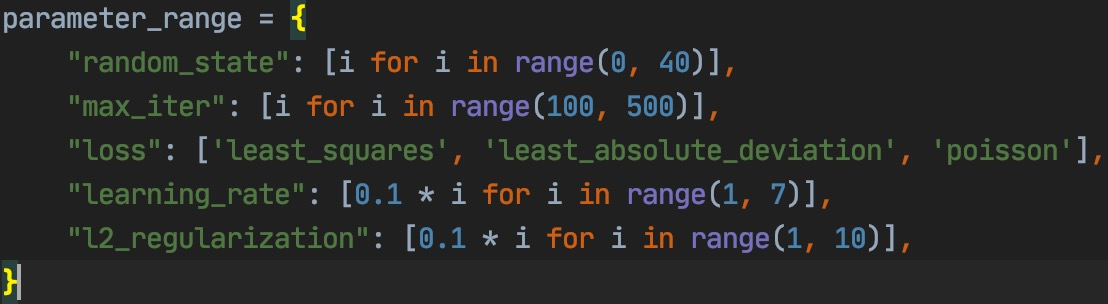
\includegraphics[width=12cm,height=5cm]{figure5.jpg}
\caption{Parameter Range}
\end{figure}

And the best result is given by parameters in table 4.
\begin{table}[h]
\centering
\begin{tabular}{|c|c|c|c|c|c|}
\hline
random\_state & max\_iter & loss           & learning\_rate & l2\_regularization & RMSE    \\ \hline
1             & 331       & least\_squares & 0.4            & 0.2                & 0.39356 \\ \hline
\end{tabular}
\caption{Best Result}
\label{tab:my-table}
\end{table}

For the suboptimal parameters, we can easily find out the performance is worse than the optimal parameters in table 5.
\begin{table}[h]
\centering
\begin{tabular}{|c|c|c|c|c|c|}
\hline
random\_state & max\_iter & loss                       & learning\_rate & l2\_regularization & RMSE    \\ \hline
4             & 415       & least\_absolute\_deviation & 0.4            & 0.8                & 0.41585 \\ \hline
39            & 175       & least\_absolute\_deviation & 0.3            & 0.7                & 0.42124 \\ \hline
32            & 368       & least\_absolute\_deviation & 0.5            & 0.7                & 0.41404 \\ \hline
3             & 177       & least\_squares             & 0.1            & 0.6                & 0.40113 \\ \hline
19            & 470       & least\_squares             & 0.1            & 0.8                & 0.42124 \\ \hline
5             & 177       & least\_absolute\_deviation & 0.2            & 0.1                & 0.42302 \\ \hline
38            & 267       & least\_absolute\_deviation & 0.2            & 0.6                & 0.42480 \\ \hline
\end{tabular}
\caption{Result of Different Hyperparameter }
\label{tab:my-table}
\end{table}

\section{PySpark implementation (optional)}
Nowadays the scale of data is growing rapidly with the development of digital technology. We decide to use pyspark to accelerate the process of  processing data. In this project, given that the operation of processing data is complex such as split the words by “~~” and compute the weighted sum value of a row. So we implement a function which compute the mean value of an column in the pandas data frame. The first step is to temporarily store the data frame as a .csv file. Then initialize a SparkSession called the Spark. Use the Spark to read the data from csv file and create an view called train. At this point, we use  SQL query to acquire the mean value of the columns and output the result to json format. At last, we read the mean value from the json. 
\end{document}

%\begin{lstlisting}
%\end{lstlisting}

%$\frac{}{}$

